\documentclass[12pt]{exam}
\usepackage{amsthm}
\usepackage{libertine}
\usepackage[utf8]{inputenc}
\usepackage[margin=1in]{geometry}
\usepackage{amsmath,amssymb}
\usepackage{multicol}
\usepackage[shortlabels]{enumitem}
\usepackage{siunitx}
\usepackage{cancel}
\usepackage{graphicx}
\usepackage{pgfplots}
\usepackage{listings}
\usepackage{tikz}


\pgfplotsset{width=10cm,compat=1.9}
\usepgfplotslibrary{external}
\tikzexternalize

\newcommand{\class}{Física II - Complementaria} % This is the name of the course 
\newcommand{\examnum}{Tarea 4} % This is the name of the assignment
\newcommand{\examdate}{27/11/2022} % This is the due date
\newcommand{\timelimit}{}





\begin{document}
\pagestyle{plain}
\thispagestyle{empty}

\noindent
\begin{tabular*}{\textwidth}{l @{\extracolsep{\fill}} r @{\extracolsep{6pt}} l}
\textbf{\class} & \textbf{Nombre:} & \textit{David Santiago Pachon Ballen}\\ %Your name here instead, obviously 
\textbf{\examnum} && \textit{Sergio Montoya Ramírez}\\
\textbf{\examdate} &&\\
\end{tabular*}\\
\rule[2ex]{\textwidth}{2pt}
% ---

\section*{2.}
El alambre y la espira rectangular están sobre el mismo plano. La corriente en
el alambre largo y recto AB que se muestra en la figura, va hacia arriba. En el
instante en que la corriente es I.
\begin{figure}[h]
    \caption{Fígura del ejercicio}
    \centering
    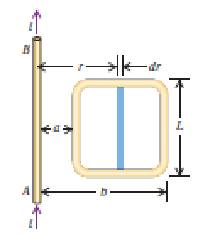
\includegraphics[width=0.2\textwidth]{Tarea_4_Punto2.png}
    \end{figure}
\begin{enumerate}
    \item ¿cuáles son la magnitud y la dirección del campo a una distancia r a la derecha del alambre?
    
    \textbf{Solución:} Como vemos el cable AB es un cable largo y por tanto todos los vectores se van a cancelar hasta hacer que
    la dirección del campo sea perpendicular al cable y podemos construir una superficie gausiana con forma de cilindro
    al rededor del cable y con radio en la base r. Por lo tanto se crean 3 superficies de las cuales solo 1 (la que rodea) tienen
    campo pues en la vertical se cancelan como dijimos previamente. con esto podemos aplicar la ley de Gauss que es 
    $$\oint \vec{E}\cdot d\vec{A}=\frac{Qin}{\varepsilon_0}$$
    como es paralelo nos queda $$\oint Ed\vec{A}=\frac{Q_in}{\varepsilon_0}=E\oint d\vec{A}$$
    y por ende podemos desarrollar de la siguiente forma:
    \begin{align*}
        &E\oint d\vec{A} = E(2\pi r l)\\
        & E(2\pi r l) = \frac{Q_in}{\varepsilon_0}\\
        &\lambda = \frac{Q}{l}\\
        &\lambda l = Q\\
        &E(2\pi r l) = \frac{\lambda l}{\varepsilon_0}\\
        &E = \frac{\lambda}{2 \pi r \varepsilon_0}\\
        &E = \frac{\lambda}{(2\pi\varepsilon_0)r}
    \end{align*}
    \item ¿Cuál es el flujo total a través de la espira?
    
    \textbf{Solución:}Como el campo magnetico esta entrando al plano. Entonces debemos encontrar la integral de superficie. En nuestro caso,
    dado que el cable es largo entonces lo unico que importa es r (la distancia al cable).Razon por la cual nos quedara su
    diferencial de superficie como $d\vec{s} = l dr \vec{i}$. Por lo tanto nos queda. 
    \begin{align*}
        &\phi_m = \int \frac{\lambda}{2\pi\varepsilon_0 r}\vec{-i}\cdot bdr\vec{i}\\
        &\text{Como la espira inicia con $r=a$ y termina con} \\
        &\text{$r=b$ esos son nuestros limites de integración}\\
        &\phi_m = -\frac{l\lambda}{2\pi\varepsilon_0}\int \frac{dr}{r}\\
        &\phi_m = -\frac{l\lambda}{2\pi\varepsilon_o}\ln{\left(\frac{b}{a}\right)}
    \end{align*}
    \item Si la corriente disminuye a una razón constante $\frac{dI}{dt}$ ¿Cuál es la fem inducida en la espira?
    
    \textbf{Solución:} Segun la ley de Faraday y lo visto en clase $f.e.m = \frac{dI}{dt}\phi_m$ y como $\phi_m$ lo calculamos justo
    en el punto anterior entonces el resultado es $$-\frac{l\lambda}{2\pi\varepsilon_o}\ln{\left(\frac{b}{a}\right)}\frac{dI}{dt}$$
    \item Cual es la dirección de la corriente inducida. 
    
    \textbf{Solución:} Dada la ley de Lenz sabemos que el sentido de la corriente inducida es tal que tiende a contrarrestar
    el flujo magnetico. Como lo calculamos en el item (2) sabemos que el campo magnetico va entrando y por tanto se debe generar
    una corriente saliente y por ley de la mano derecha sabemos que la corriente va a seguir unsentido antihorario.
    \item Ahora cual es la fuerza magnética sobre la espira de corriente
    
    \textbf{Solución: } Como estamos en un rectangulo entonces podemos saber que la fuerza sobre la espira es 
    $$\vec{F} = \vec{F}_{12} + \vec{F}_{23} + \vec{F}_{34} + \vec{F}_{41}$$ En este caso utilizando el campo calculado en
    la sección (2) entonces sabemos que 
    $$F_{41} = I \int_{41} d l \times B_1(x)$$
    y por la ubicación de este segmento nos queda
    $$F_{41} = I \int_a^b dx \vec{i}\times \frac{\lambda}{(2\pi\varepsilon_0)x}$$
    $$F_{41} = \frac{\lambda I_2 I_1}{(2\pi\varepsilon_0)}(j)\int_a^b \frac{dx}{x} = \frac{\lambda I_1 I_2}{(2\pi\varepsilon_0)}(\vec{j})\ln(\frac{b}{a})$$
    Si repetimos el proceso con $F_{23}$ nos queda
    \begin{align*}
        F_{41} = I \int_{41} d l \times B_1(x)\\
        F_{41} = I \int_a^b dx -\vec{i}\times \frac{\lambda}{(2\pi\varepsilon_0)x}\\
        F_{41} = \frac{\lambda I_1 I_2}{(2\pi\varepsilon_0)}(j)\int_a^b \frac{dx}{x} = \frac{\lambda I_1 I_2}{(2\pi\varepsilon_0)}(-\vec{j})\ln(\frac{b}{a})
    \end{align*}
    Ahora bien, calculando la fuerza sobre el tramo $F_{12}$ y $F_{34}$ nos quedara
    \begin{align*}
        &F_{12} = I \int_0^L dy(-j)\times \frac{\lambda}{(2\pi\varepsilon_0)r}\\
        &F_{12} = \frac{\lambda I_1 I_2}{(2\pi\varepsilon_0)r} \int dy = \frac{\lambda I_1 I_2}{(2\pi\varepsilon_0)a} (i)
    \end{align*}
    Y para $F_{34}$
    \begin{align*}
        &F_{34} = I \int_0^L dy(j)\times \frac{\lambda}{(2\pi\varepsilon_0)r}\\
        &F_{34} = -\frac{\lambda I_1 I_2}{(2\pi\varepsilon_0)r} \int dy = -\frac{\lambda I_1 I_2}{(2\pi\varepsilon_0)b} (i)
    \end{align*}
    Como las corrientes solo dependen de la distancia a el hilo y esta es igual y ademas las fuerzas $F_{41}$ y $F_{23}$ se cancelan
    entonces al sumar nos queda $$F = \frac{\lambda I_1 I_2}{(2\pi\varepsilon_0)a} (i) -\frac{\lambda I_1 I_2}{(2\pi\varepsilon_0)b} (i)$$
    o lo que es lo mismo $$F = \frac{\lambda I_1 I_2}{(2\pi\varepsilon_0)}(\frac{1}{a}-\frac{1}{b})(i)$$
\end{enumerate}


\end{document}
